\newcommand{\adag}[1]{\hat{a}_{#1}^\dagger}
\newcommand{\aop}[1]{\hat{a}_{#1\vphantom{\dagger}}}
\chapter{Theory: Background}
This chapter will cover the elementary concepts required to describe an membrane based optomechanical system in a quantum regime. We will first recall basics on optical field quantization as well describing coherent and squeezed light field, to then turn to the more specific frequency dependent squeezed light field. Secondly, we will cover the mathematical description of a mechanical resonator interacting with a generic coherent optical field, highlighting the differences with the seminal optomechanical system of a mirror on a spring. Finally, we will derive the equations of motions of a membrane based optomechanical system with frequency dependent squeezed optical fields. 
\minitoc
\newpage
\section{Quantum Optics}
\subsection{Quantum Description of Light}

\subsubsection{Quantised Electromagnetic Field}
% \the\textwidth
We consider the quantised electromagnetic field in a volume $V$. The electric field operator can be written as  
\begin{equation}
\hat{\mathbf{E}}(\mathbf{r}, t) 
= i \sum_{\ell} \mathcal{E}_\ell 
\left[ \hat{a}^{\vphantom{\dagger}}_{\ell}\,\mathbf{f}_{\ell}(\mathbf{r})\,e^{-i\omega_{\ell} t} 
- \hat{a}_{\ell}^\dagger\,\mathbf{f}_{\ell}^*(\mathbf{r})\,e^{+i\omega_{\ell} t} \right],
\end{equation}
where   $\mathcal{E}_l = \sqrt{\frac{\hbar \omega_l}{2 \varepsilon_0 V}}$ is the field amplitude per photon in mode $\ell$, $\hbar$ is the reduced Planck constant, $\omega_\ell$ is the angular frequency of mode $\ell$, and $\varepsilon_0$ is the vacuum permittivity. The spatial mode functions $\mathbf{f}_{\ell}(\mathbf{r})$ form an orthonormal basis in $V$ according to  
\begin{equation*}
\int_V d^3r\; \mathbf{f}_{\ell}^*(\mathbf{r}) \cdot \mathbf{f}_{\ell'}(\mathbf{r}) 
= \delta_{\ell \ell'} .
\end{equation*}
The annihilation and creation operators $\hat{a}_{\ell}(t)$ and $\hat{a}_{\ell}(t)^\dagger$ satisfy the canonical commutation relations  
\[
[\hat{a}_{\ell}^{\vphantom{\dagger}}, \hat{a}_{\ell'}^\dagger] = \delta_{\ell \ell'} \,, \quad
[\hat{a}_{\ell}^{\vphantom{\dagger}}, \hat{a}_{\ell'}^{\vphantom{\dagger}} ] = 0, \quad [\hat{a}_{\ell}^\dagger, \hat{a}_{\ell'}^\dagger] = 0  
\]
The explicit time dependence of the operators allows one to describe both slow classical modulations of the field and the intrinsic quantum fluctuations.

\subsubsection{Fock basis}
In this description of the optical field, each mode $\ell$ is modeled as a quantum harmonic oscillator with a discrete set of energy eigenstates known as \textit{Fock states} or number states, denoted $\ket{n_\ell}$. These states form an orthonormal basis and satisfy $\hat{n}_{\ell} \ket{n_\ell} = n_\ell \ket{n_\ell}$, where $\hat{n}_{\ell}$ is the number operator defined by
\[
\hat{n}_{\ell} = \hat{a}_{\ell}^\dagger \hat{a}^{\vphantom{\dagger}}_{\ell}.
\]
The action of the creation and annihilation operators on these states is given by
\[
\hat{a}^{\vphantom{\dagger}}_{\ell} \ket{n_\ell} = \sqrt{n_\ell} \ket{n_\ell - 1}, \quad
\hat{a}_{\ell}^\dagger \ket{n_\ell} = \sqrt{n_\ell + 1} \ket{n_\ell + 1}.
\]
They allow transitions between Fock states by lowering or raising the photon number in mode $\ell$ by one unit. The vacuum state $\ket{0_\ell}$ is annihilated by $\hat{a}^{\vphantom{\dagger}}_{\ell}$, satisfying $\hat{a}^{\vphantom{\dagger}}_{\ell} \ket{0_\ell} = 0$. Thus, the Hamiltonian for the electromagnetic field becomes a sum of harmonic oscillator energies:
\begin{equation}
\hat{H} = \sum_\ell \hbar \omega_{\ell} \, \hat{a}_{\ell}^\dagger \hat{a}^{\vphantom{\dagger}}_{\ell} 
\end{equation}
where we ignore the constant zero-point energy term $\frac{1}{2} \hbar \omega_{\ell}$ for simplicity. \\

In the following parts, we will always focus on a single mode of the electromagnetic field unless stated otherwise (for the mode matching part), which is sufficient to illustrate the concepts of quantum optics and optomechanics. The generalization to multiple modes is straightforward and follows the same principles. The electrif field operator is then written
\begin{equation}
\hat{\mathbf{E}}(\mathbf{r}, t)
= i \mathcal{E}_0
\left[ \hat{a}^{\vphantom{\dagger}}\,\mathbf{f}(\mathbf{r})\,e^{-i\omega_0 t}
- \hat{a}^\dagger\,\mathbf{f}^*(\mathbf{r})\,e^{+i\omega_0 t} \right].
\end{equation}


\subsubsection{Quadrature Operators}
We describe the phase-space properties of a field mode using hermitian quadrature operators. These are linear combinations of the annihilation and creation operators that correspond to measurable observables in the electromagnetic field. The two most common quadratures are defined as follows:
\begin{equation}
\mathbf{\hat{a}}\;\equiv\;
\begin{pmatrix}\hat a_1\\[2pt]\hat a_2\end{pmatrix}
=\mathbf\Gamma \, \mathbf{\hat{u}}, \label{II.2}
\qquad
\mathbf \Gamma \equiv
\begin{pmatrix}
1 & 1 \\
-i & i
\end{pmatrix},
\quad
\mathbf{\hat{u}}\;\equiv\;
\begin{pmatrix}\hat a\\ \hat a^\dagger\end{pmatrix}
\end{equation}
where we defined the field vector $\mathbf{\hat{u}}$ and the transfer matrix $\mathbf \Gamma$, later used to switch from One-Photon to Two-Photon description of optical elements. In components, we then have $\hat a_1=\hat a^\dagger+\hat a$ and $\hat a_2=i(\hat a^\dagger-\hat a)$.
The matrix form commutator reads
\begin{equation}
[\mathbf{\hat{u}}, \mathbf{\hat{u}}^{\dagger}] = \mathbf{\sigma_z}, 
\end{equation}
with $\sigma_z$ the Pauli Z matrix. 
An arbitrary rotated quadrature pair is obtained by
\begin{equation}
\mathbf{\hat{a}_\phi}\;\equiv\;
\begin{pmatrix}\hat a_\phi\\[2pt]\hat a_{\phi+\pi/2}\end{pmatrix}
= \mathbf R(\phi)\,\mathbf{\hat{a}}
= \mathbf R(\phi)\,\mathbf\Gamma \,\mathbf{\hat{u}},
\qquad
 \mathbf R(\phi)\equiv
\begin{pmatrix}
\cos\phi & \sin\phi \\
-\sin\phi & \cos\phi \label{II.4}
\end{pmatrix}.
\end{equation}
We notice than 
\begin{equation}
\mathbf R(\phi)\,\boldsymbol{\Gamma}
=
\begin{pmatrix}
\cos\phi & \sin\phi \\
-\sin\phi & \cos\phi
\end{pmatrix}
\begin{pmatrix}
1 & 1 \\
-i & i
\end{pmatrix}
=
\begin{pmatrix}
e^{-i\phi} & e^{i\phi} \\[4pt]
-\,i\,e^{-i\phi} & \;\;i\,e^{i\phi}
\end{pmatrix}.
\end{equation}
so that in components we have 
\begin{equation}
\begin{alignedat}{3}
\hat a_\phi \;&=\;& \hat a_1 \cos\phi + \hat a_2 \sin\phi \;&= \hat a\,e^{-i\phi} + \hat a^\dagger\,e^{+i\phi}\\
\hat a_{\phi+\pi/2} \;&=\;& -\hat a_1 \sin\phi + \hat a_2 \cos\phi \;&= i\!\left(\hat a^\dagger\,e^{+i\phi} - \hat a\,e^{-i\phi}\right).
\end{alignedat}
\end{equation}
The commutators of the rotated quadrature operators read
\begin{equation}
\begin{aligned}
[\hat{\mathbf{a}}_\phi , \hat{\mathbf{a}}_\phi^{\dagger}]
&= \mathbf R(\phi) \mathbf \Gamma\,[\hat{\mathbf{u}},\hat{\mathbf{u}}^{\dagger}]\, \mathbf \Gamma^{\dagger} \mathbf R^{\dagger}(\phi) \\[4pt]
&= \mathbf R(\phi)\mathbf \Gamma \mathbf \sigma_z \mathbf \Gamma^{\dagger} \mathbf R^{\dagger}(\phi) \\[4pt]
&= 2i\, \mathbf R(\phi) \mathbf J \mathbf R^{\dagger}(\phi) \\[4pt]
&= 2i\,\mathbf J,
\end{aligned}
\end{equation}
where $\mathbf{J}$ is the symplectic form defined as
\begin{equation}
\mathbf{J} \equiv
\begin{pmatrix}
0 & 1 \\
-1 & 0
\end{pmatrix}.
\end{equation}
Note that since $\hat{\mathbf{a}}_\phi$ is hermitian, we have $\hat{\mathbf{a}}_\phi^\dagger = \hat{\mathbf{a}}_\phi^T$, and similarly $\mathbf{R^\dagger(\phi)} = \mathbf{R}^T(\phi)$ since all its entries are real. \\ 
\\
This compact vector form will be used later for the One- and Two-Photon description of the light field behaviours in optomechanical systems with squeezed light input. \\
\noindent \textbf{Note:} \color{red} notes the fact that these are defined for a specific $\ell$, so at each mode is associated such a quadrature vector. The multimode treatment is used by the multimode quantum optics community, notably to describe mutimode non gaussian states, hidden squeezing (beyond homodyne detection correlations, Patera and co) \color{black}
\subsubsection{Linearization of the optical field}

The annihilation operator can be decomposed as
\begin{equation}
\begin{split}
    \hat{a} & = \langle \hat{a} \rangle + \delta\hat{a}\\
    & = \bar{\alpha} + \delta\hat{a} \\
\end{split}
\label{II.8}
\end{equation}
where \(\langle \hat{a} \rangle = \bar{\alpha} \in \mathbb{C}\) is the mean complex amplitude of the quantum state, and \(\delta\hat{a}\) represents quantum fluctuations with \(\langle \delta\hat{a}\rangle = 0\). Note this decomposition is valid for any quantum state, including coherent and squeezed states. We note $\bar{\alpha}$ to distinguish it from the complex amplitude $\alpha$ of a coherent state introduced below, which is a specific case of this decomposition. The associated matrix form is 
\begin{equation}
\mathbf{\hat{u}} =  \begin{pmatrix} \bar{\alpha}  \\ \bar{\alpha}^*  \end{pmatrix} + \begin{pmatrix} \delta\hat{a} \\ \delta\hat{a}^\dagger \end{pmatrix} =  \mathbf{\bar{u}} + \mathbf{\delta \hat{u}}
\end{equation}
and it then follows that fluctuations in the quadrature operators can be expressed as
\begin{equation}
  \mathbf{\delta \hat{a}_\phi} = \mathbf{R}(\phi) \, \mathbf\Gamma  \, \mathbf{\delta \hat{u}}
\end{equation}
They also retain the canonical commutation relations
\begin{equation}
[\mathbf{\delta \hat{u}}, \mathbf{\delta \hat{u}}^{\dagger}] = \mathbf{\sigma_z} \qquad \Rightarrow \qquad
[\mathbf{\delta \hat{a}_\phi}, \mathbf{\delta \hat{a}_\phi}^{T}] = 2i\,\mathbf{J}.
\label{II.11}
\end{equation}

\noindent \textbf{Note:} \color{red} notes on first and second moments, as well as beyond second moments correlations and their use i.e. when and why is this linearization ok to use etc etc \color{black}

\subsubsection{Heisenberg Uncertainty Relation }
The covariance of Hermitian operators \(\hat{A}\) and \(\hat{B}\) is defined as
\begin{equation}
    \mathrm{Cov}(\hat{A},\hat B) = \tfrac12 \big\langle \{ \delta\hat{A}, \delta\hat{B} \} \big\rangle \\
\end{equation}
Now if $\hat{A}=\hat{B}$ this is the variance written as 
\begin{equation}
    \Delta A^2 = \langle {(\delta \hat{A})^2} \rangle
\end{equation}
Considering the quadrature operators, we define the covariance matrix as
\begin{equation}
\mathbf{V_\phi} \equiv \tfrac12 \big\langle \{  \mathbf{\delta \hat{a}_\phi},  \mathbf{\delta \hat{a}_\phi}^{\,T} \} \big\rangle
= \begin{pmatrix}
\Delta \hat{a}_\phi^2 &
\mathrm{Cov}(\hat{a}_\phi,\hat{a}_{\phi+\pi/2}) \\[4pt]
\mathrm{Cov}(\hat{a}_\phi,\hat{a}_{\phi+\pi/2})  &
\Delta \hat{a}_{\phi+\pi/2}^2
\end{pmatrix}
\end{equation}
and the Heisenberg uncertainty relation reads as
\begin{equation}
  \det \mathbf{V_\phi} \geq 1 \qquad \Rightarrow \qquad \Delta \hat{a}^2_\phi \Delta \hat{a}^2_{\phi+\pi/2} - \mathrm{Cov}^2(\hat{a}_\phi,\hat{a}_{\phi+\pi/2})\geq 1
\end{equation}

\subsection{Coherent and Squeezed States}
We now turn to standard optical quantum states, in particular gaussian states i.e.\ full positive in Wigner function representations such as coherent and squeezed states, that we will denote in braket notation as $|\alpha\rangle$ and $|\alpha,r, \theta\rangle $.
\subsection*{Coherent States:}
The coherent state $\ket{\alpha}$ is an eigenstate of the annihilation operator:
\begin{equation}
\hat{a}\ket{\alpha} = \alpha \ket{\alpha}
\label{II.14}
\end{equation}
where $\alpha = |\alpha| e^{i\bar{\varphi}}$ is a complex number representing the mean coherent amplitude. In this notation, the angle $\bar{\varphi}$ is the mean angle of the distribution, used to describe the relative phase to a reference (e.g. a local oscillator). The $\hat{a}$ linear decomposition above (Eq~\eqref{II.8}) then yields $\alpha = \bar{\alpha}$ for a coherent state. It can be expressed in the Fock basis as
\begin{equation}
\ket{\alpha} = e^{-|\alpha|^2/2} \sum_{n=0}^\infty \frac{\alpha^n}{\sqrt{n!}}\,\ket{n}
\label{II.15}
\end{equation}
and are generated by the action of the displacement operator $\hat{D}(\alpha)$ on the vacuum state $\ket{0}$:
\begin{equation}
\ket{\alpha} = \hat{D}(\alpha)\ket{0},\qquad \hat{D}(\alpha) = \exp\!\left(\alpha \hat{a}^\dagger - \alpha^* \hat{a}\right)
\label{II.16}
\end{equation}
\noindent \textbf{Note:} \color{red} note on the convention used i.e. $\alpha \neq \bar{\alpha}$, $\alpha_0 \neq \bar{\alpha}_0$ \color{black}
\subsubsection*{Expectation values of quadrature operators}

Using the quadrature vector $\hat{\mathbf a} = (\hat{a}_1,\,\hat{a}_2)^T = \Gamma (\hat{a}, \hat{a}^\dagger)^T$ given in Eq~\eqref{II.2}, the expectation values in a coherent state are
\begin{equation}
\langle \hat{\mathbf a} \rangle
= \Gamma
\begin{pmatrix}\alpha\\ \alpha^*\end{pmatrix}
= \begin{pmatrix}
\alpha+\alpha^* \\[2pt]
i(\alpha^*-\alpha)
\end{pmatrix}
= 2\begin{pmatrix}
\mathrm{Re}\,\alpha \\[2pt]
\mathrm{Im}\,\alpha
\end{pmatrix}.
\label{II.CS.1}
\end{equation}
For a quadrature rotated by an angle $\phi$ (Eq~\ref{II.4}),
\begin{equation}
\langle \hat{\mathbf a}_\phi\rangle
= \mathbf R(\phi)\,\langle \hat{\mathbf a}\rangle
=
2\begin{pmatrix}
\mathrm{Re}\big(\alpha e^{-i\phi}\big) \\[2pt]
\mathrm{Im}\big(\alpha e^{-i\phi}\big)
\end{pmatrix}.
\end{equation}


\subsubsection*{Amplitude and phase quadratures}

It is convenient to introduce the amplitude-phase quadrature vector at $\phi = \bar{\varphi}$
\begin{equation}
\hat{\mathbf a}_{\bar{\varphi}} =
\begin{pmatrix}
\hat{p} \\[2pt]
\hat{q}
\end{pmatrix}
=
\begin{pmatrix}
\hat{a}_{\bar{\varphi}} \\[2pt]
\hat{a}_{\bar{\varphi}+\pi/2}
\end{pmatrix}.
\end{equation}
with expectation values
\begin{equation}
\langle \hat{\mathbf a}_{\bar{\varphi}} \rangle
=
2\begin{pmatrix}
|\alpha| \\[2pt]
0
\end{pmatrix},
\end{equation}



\subsubsection*{Covariance matrix}
For a coherent state, fluctuations are vacuum-like:
\begin{equation}
\Delta \hat{a}_\phi^2 = \Delta \hat{a}_{\phi+\pi/2}^2 = 1,
\qquad
\mathrm{Cov}(\hat{a}_\phi,\hat{a}_{\phi+\pi/2}) = 0,
\end{equation}
so that
\begin{equation}
\mathbf V_\phi =
\begin{pmatrix}
1 & 0\\
0 & 1
\end{pmatrix}
= \mathbb{I}_2,
\quad \forall \phi .
\label{II.CS.3}
\end{equation}
This saturates the Heisenberg uncertainty relation $\det \mathbf V_\phi = 1$ in the units defined here i.e. it is a minimum uncertainty state. 

\subsubsection*{Photon number statistics}

The mean and variance of the photon number operator $\hat{N}=\hat{a}^\dagger\hat{a}$ are
\begin{equation}
\langle \hat{N} \rangle = |\alpha|^2,
\qquad
\Delta N^2 = |\alpha|^2.
\label{II.19}
\end{equation}
That is, coherent states display Poissonian photon statistics.


\begin{figure}
\centering
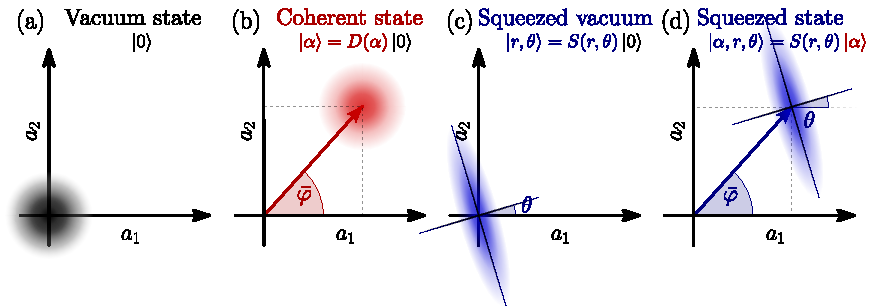
\includegraphics[width=\textwidth]{./chap2/fig/quantum_states.pdf}
\caption{Phase-space representations of quantum states and transformations.
(a) Wigner function of the vacuum state: a circular Gaussian centered at the origin, representing equal quantum fluctuations in both quadratures $a_1$ and $a_2$.
(b) Wigner function of a coherent state: a displaced circular Gaussian, showing a shift in phase space along an angle $\varphi$ with unchanged, isotropic noise.
(c) Wigner function of a squeezed vacuum state: an elliptical Gaussian centered at the origin, with reduced noise along a rotated quadrature $X_\theta$ and increased noise in the orthogonal direction.
(d) Wigner function of a displaced squeezed state: an ellipse shifted away from the origin, combining anisotropic fluctuations and a nonzero mean amplitude. The displacement angle $\varphi$ and squeezing angle $\theta$ are independent.} 
\end{figure}


\subsection*{Squeezed States:}

Squeezed states $|\alpha, r, \theta\rangle $ are quantum gaussian states of light in which the noise (variance) of one quadrature is reduced below the vacuum level, at the expense of increased noise in the conjugate quadrature. The single-mode squeezed vacuum state is defined as
\begin{align}
|0, r, \theta \rangle = \hat{S}(r, \theta) |0\rangle , \quad \hat{S}(\theta) = \exp\left[\frac{r}{2}(e^{-2 i\theta} \hat{a}^2 - e^{-2 i\theta} \hat{a}^{\dagger 2})\right]
\end{align}
where $r$ is the squeezing parameter (strength) and $\theta$ is the squeezing angle i.e. the angle along which one quadrature is reduced below vacuum level. The most general Gaussian state is the displaced squeezed state, obtained by applying both the squeezing operator $\hat{S}(r, \theta)$ and the displacement operator $\hat{D}(\alpha)$ to the vacuum:
\begin{equation}
|\alpha, r, \theta\rangle = \hat{S}(r, \theta)\hat{D}(\alpha)|0\rangle
\end{equation}
where $\hat{D}(\alpha)$ displaces the state in phase space by the complex amplitude $\alpha$, defined similarly to the coherent state. \\

\noindent \textbf{Note:}  The displacement and squeezing operators do not commute, i.e. $\hat{D}(\alpha)\hat{S}(r, \theta) \neq \hat{S}(r, \theta)\hat{D}(\alpha)$. However, both orderings correspond to experimentally valid procedures: one can either squeeze the vacuum and then displace (e.g. by mixing with a coherent state ona beamsplitter), or squeeze a coherent state straight away (e.g. by seeding an optical parametric amplifier). The resulting state is always a displaced squeezed state, but the relative phase between displacement and squeezing may differ.
% -------------------------------------------------
\subsubsection*{Expectation values of quadrature operators}

Using the usual quadratures defined in Eq~\eqref{II.2} and \eqref{II.4}, the expectation values in a displaced squeezed state are
\begin{equation}
\langle \mathbf{\hat{a}} \rangle
= 2
\begin{pmatrix}
\mathrm{Re}\,\alpha \\[2pt]
\mathrm{Im}\,\alpha
\end{pmatrix}, 
\qquad
\langle \mathbf{\hat{a}_\phi} \rangle
= 2
\begin{pmatrix}
\mathrm{Re}\!\left(\alpha e^{-i\phi}\right) \\[2pt]
\mathrm{Im}\!\left(\alpha e^{-i\phi}\right)
\end{pmatrix}.
\label{II.xx3}
\end{equation}
For a squeezed vacuum ($\alpha=0$) all quadrature means vanish.

\subsubsection*{Quadrature aligned with the squeezing axis \color{red} to rewrite \color{black}}

Choosing $\phi = \theta$ yields
\begin{equation}
\Delta \hat a_\theta^2 = e^{-2r}, \qquad
\Delta \hat a_{\theta+\pi/2}^2 = e^{2r}, \qquad
\mathrm{Cov}(\hat a_\theta, \hat a_{\theta+\pi/2}) = 0,
\end{equation}
with uncertainty product $\Delta \hat a_\theta\, \Delta \hat a_{\theta+\pi/2} = 1$ saturating the Heisenberg bound.
The corresponding mean vector is
\begin{equation}
\langle \mathbf{\hat{a}_\theta} \rangle
= 2
\begin{pmatrix}
\mathrm{Re}(\alpha e^{-i\theta}) \\[2pt]
\mathrm{Im}(\alpha e^{-i\theta})
\end{pmatrix}.
\label{II.xx7}
\end{equation}

\begin{figure}
\centering
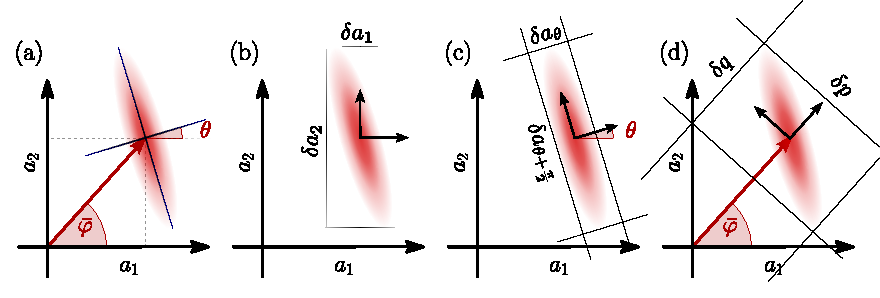
\includegraphics[width=\textwidth]{./chap2/fig/quantum_quadraturesBis.pdf}
\caption{Phase-space representations of quantum states and transformations.
(a) Wigner function of the vacuum state: a circular Gaussian centered at the origin, representing equal quantum fluctuations in both quadratures $X_1$ and $X_2$.
(b) Wigner function of a coherent state: a displaced circular Gaussian, showing a shift in phase space along an angle $\varphi$ with unchanged, isotropic noise.
(c) Wigner function of a squeezed vacuum state: an elliptical Gaussian centered at the origin, with reduced noise along a rotated quadrature $X_\theta$ and increased noise in the orthogonal direction.
(d) Wigner function of a displaced squeezed state: an ellipse shifted away from the origin, combining anisotropic fluctuations and a nonzero mean amplitude. The displacement angle $\varphi$ and squeezing angle $\theta$ are independent.} 
\end{figure}
% -------------------------------------------------
\subsubsection*{Covariance matrix}

Let $\psi \equiv \phi - \theta$ be the measurement angle $\phi$ relative to the squeezing axis $\theta$.  
For a displaced squeezed state, the covariance matrix is
\begin{equation}
\mathbf{V}_\phi = \mathbf R(\psi)
\begin{pmatrix}
e^{-2r} & 0 \\[2pt]
0 & e^{2r}
\end{pmatrix}
\mathbf R(\psi)^{T}.
\label{II.xx4}
\end{equation}
Expanding this explicitly gives
\begin{equation}
\mathbf{V}_\phi =
\begin{pmatrix}
e^{-2r} \cos^2\!\psi + e^{2r} \sin^2\!\psi 
& \frac{1}{2} \sin 2\psi \,\left(e^{2r} - e^{-2r}\right) \\[6pt]
\frac{1}{2} \sin 2\psi \,\left(e^{2r} - e^{-2r}\right) 
& e^{-2r} \sin^2\!\psi + e^{2r} \cos^2\!\psi
\end{pmatrix}.
\label{II.xx5}
\end{equation}
The covariance term is therefore
\begin{equation}
\mathrm{Cov}(\hat a_\phi, \hat a_{\phi+\pi/2})
= \frac{1}{2} \sin 2(\phi-\theta)\, \left(e^{2r} - e^{-2r}\right),
\label{II.xx6}
\end{equation}
which vanishes when $\sin 2(\phi-\theta) = 0$, i.e.
\begin{equation*}
\phi - \theta \in \left\{ 0, \frac{\pi}{2}, \pi, \ldots \right\}.
\end{equation*}
Along these principal axes of squeezing, $\mathbf{V}_\phi$ is diagonal. 

\subsubsection{Amplitude and Phase squeezed states}
Considering a displaced squeezed state, two special cases are of interest: the amplitude squeezed state where $\theta=\bar{\varphi}$ and the phase squeezed state where $\theta = \bar{\varphi}+\pi/2$. In the first case, the amplitude quadrature $\hat{p}$ is squeezed, while the phase quadrature $\hat{q}$ is anti-squeezed. In the second case, the phase quadrature is squeezed, while the amplitude quadrature is anti-squeezed. The covariance matrices for these states can be derived from Eq.~\eqref{II.xx4} by setting $\psi = 0$ or $\psi = \pi/2$, respectively.
\subsubsection*{Photon number statistics}

The mean and variance of the photon number operator $\hat N = \hat a^\dagger \hat a$ in a displaced squeezed state are
\begin{equation}
\langle \hat N \rangle = |\alpha|^2 + \sinh^2 r,
\qquad
\Delta N^2 = |\alpha|^2 \cosh 2r + \frac{1}{2} \sinh^2 2r.
\label{II.xx8}
\end{equation}
\color{red}
to rewrite
\color{black}
This shows that the squeezing operation increases the mean photon number of the coherent state by adding photons. Physically, this reflects the fact that generating squeezed light requires injecting energy into the system, so the squeezed vacuum contains correlated field excitations (photons) in even numbers. This is further seen by examining the photon-number distribution $P_n$: for a squeezed vacuum only even $n$ occur, while displacement progressively repopulates the odd $n$ and shifts weight to higher $n$, in agreement with the increase of $\langle \hat{N} \rangle$ and $\Delta N^2$ above.



\color{black}

\subsection{Sidebands and Quantum Noises}

\subsubsection{Modulation picture}
In realistic optical systems, the electromagnetic field is never perfectly monochromatic, nor isolated from its environment, nor static through time. Instead, it exhibits a finite spectral linewidth (stimulated emission, phase noise etc...), as well as non intentional/intentional modulations, all imprinted onto the carrier field. These effects cause the field amplitude and phase to evolve slowly compared to the optical frequency $\omega_0$. \\

As a result, the complex amplitude associated with each mode and described by the Schrodinger-picture annihilation operator $\hat{a}$, acquires an explicit time dependence beyond the standard fast-oscillating term $e^{-i\omega_0 t}$. It is often quoted as \textit{modulation} picture in the litterature. We then promote the field vector to 
\begin{equation}
\mathbf{\hat{u}}= \mathbf{\bar{u}} + \mathbf{\delta \hat{u}} \quad \rightarrow \quad
  \mathbf{\hat{u}}(t)=
 \mathbf{\bar{u}}(t) + \mathbf{\delta \hat{u}(t)}
\end{equation}
where the canonical commutation relations given in equation~\eqref{II.11} becomes:
\begin{equation}
  [\delta\mathbf{\hat{u}}(t), \delta \mathbf{\hat{u}}(t')^{\dagger}] = \mathbf{\sigma_z} \, \delta (t-t').
\end{equation}
This time dependence allows us to track both slow classical modulations of the field $\mathbf{\bar{u}}(t)$ and the intrinsic quantum fluctuations $\mathbf{\delta \hat{u}(t)}$. Note this is equivalent to the interaction picture where the reference angular frequency would be $\omega_0$, but where we also consider dynamical processes way slower than this frequency. Additionally, we will always consider the limit of weak fluctuations, where the quantum noise can be treated perturbatively around the classical field i.e. 
\[
|\bar{\alpha}(t)| \gg \Delta \hat a_\theta(t)
\]
The resulting field operator can then be expressed as a 
\begin{equation}
\begin{aligned}
\hat{\mathbf{E}}(\mathbf{r}, t) 
=i  \mathcal{E}_0 \bigg[ & \left[ \alpha(t)\, \mathbf{f}(\mathbf{r})\, e^{-i \omega_0 t} 
- \alpha^*(t)\, \mathbf{f}^*(\mathbf{r})\, e^{i \omega_0 t} \right] \\
\quad +  &\left[ \delta \hat{a}(t)\, \mathbf{f}(\mathbf{r})\, e^{-i \omega_0 t}
- \delta \hat{a}^\dagger(t)\, \mathbf{f}^*(\mathbf{r})\, e^{i \omega_0 t} \right] \bigg]
\end{aligned}
\end{equation} 

\subsubsection{Fourier Domain \& Sidebands}
To deal with noise spectra, we need to rewrite the various quadratures defined in the previous sections in the Fourier domain, where each frequency component is called a \textit{sideband}. The Fourier transform of the field vector is defined as
\begin{equation}
  \begin{split}
    \mathbf{\hat{u}}[\Omega] &= \frac{1}{\sqrt{2\pi}}\int_{\infty}^{-\infty}  dt \, e^{i\Omega t} \, \mathbf{\hat{u}}(t)\\
\mathbf{\hat{u}}(t) &= \frac{1}{\sqrt{2\pi}}\int_{\infty}^{-\infty}  d\Omega \, e^{-i\Omega t} \, \mathbf{\hat{u}}[\Omega]
  \end{split}
\end{equation}
where $\Omega \ll \omega_0$ is the sideband frequency relative to the so called \textit{carrier} frequency $\omega_0$. In this definition, a notable property is that the hermitian conjugate in the time domain translates to a frequency inversion in the Fourier domain:
\begin{equation}
   \Big[\hat{a}(t)\Big]^{\dagger} = \hat{a}^\dagger(t),  \quad
   \Big[\hat{a}[\Omega]\Big]^{\dagger}  = \hat{a}^\dagger[-\Omega].
\end{equation}
Carrying out the linearization in the Fourier domain, we have
\begin{equation}
  \begin{split}
      \mathbf{\hat{u}}[\Omega] &= \begin{pmatrix} \hat{a}[\Omega] \\ \hat{a}^\dagger[-\Omega] \end{pmatrix}  \\
       & = \begin{pmatrix} \bar{\alpha}[\Omega] \\ \bar{\alpha}^*[-\Omega] \end{pmatrix} + \begin{pmatrix} \delta\hat{a}[\Omega] \\ \delta\hat{a}^\dagger[-\Omega] \end{pmatrix} \\
      & = \mathbf{\bar{u}}[\Omega] + \mathbf{\delta \hat{u}}[\Omega]\\
  \end{split}
\end{equation}
with the fluctuations commutator reading
\begin{equation}
  [\delta \mathbf{\hat{u}}[\Omega], \delta \mathbf{\hat{u}}[\Omega']^{T}] = \mathbf{\sigma_z} \, \delta(\Omega + \Omega').
\end{equation}
This very way of writing the field vector is known as the \textit{two-photon} formalism, introduced by Caves and Schumaker~\cite{Caves1985,Caves1985a}. The quadrature operators in the Fourier domain are then written as 
\begin{equation}
  \begin{split}
      \mathbf{\hat{a}_\phi}[\Omega] &= \mathbf{R}(\phi) \, \mathbf{\Gamma} \, \mathbf{\hat{u}}[\Omega]\\
      & = \mathbf{R}(\phi) \, \mathbf{\Gamma} \,\mathbf{\bar{u}}[\Omega] + \mathbf{R}(\phi) \, \mathbf{\Gamma} \, \mathbf{\delta \hat{u}}[\Omega] \\
      & = \underbrace{2|\bar{\alpha}| \begin{pmatrix}
  \cos(\bar{\varphi}-\phi) \\[2pt]
  \sin(\bar{\varphi}-\phi)
\end{pmatrix} \delta(\Omega)}_{\text{classical part}} +
\underbrace{\mathbf{R}(\phi) \, \mathbf{\Gamma} \, \mathbf{\delta \hat{u}}[\Omega]}_{\text{quantum fluctuations}}
  \end{split}
\end{equation}


\noindent\textbf{Note: }
In the modulation picture, fluctuations in the time domain appear as symmetric sidebands at \(+\Omega\) and \(-\Omega\).
Any experimentally accessible, real signal arises from the interference of these two sidebands (quadratures in homodyne detection, intensity fluctuations, photocurrent spectra); equivalently, Hermiticity in time forces Fourier components to couple \(+\Omega\) with \(-\Omega\).
Packaging the field as the two-photon vector \(\big(\hat a[\Omega],\,\hat a^\dagger[-\Omega]\big)^{\mathsf T}\) therefore groups exactly the two degrees of freedom that generate a single measurable fluctuation at frequency \(\Omega\). This makes correlations between the sidebands (which are the essence of frequency-dependent squeezing) explicit and ensures that quadrature spectra remain manifestly real. By contrast, the vector \(\big(\hat a[\Omega],\,\hat a^\dagger[\Omega]\big)^{\mathsf T}\) is convenient for per-frequency photon-number or passive-scattering calculations, but it obscures the intrinsic pairing required to form real observables, forcing one to carry \(-\Omega\) separately.
For the noise-spectral analysis pursued here, the sideband-pair representation is thus the phenomenologically natural and algebraically minimal choice.


\subsubsection*{Amplitude Modulation (AM)}

Let the classical coherent amplitude be modulated at $\Omega_{\text{mod}}$ in amplitude:
\begin{equation}
  \alpha(t) = \bar{\alpha} \left(1 + \epsilon_a \cos(\Omega_{\text{mod}} t)\right)
\end{equation}
with $\epsilon_a \ll 1$, the field amplitude modulation depth. While the DC term lives at frequency $\omega_0$, the modulation introduces sidebands at frequencies $\omega_0 \pm \Omega_{\text{mod}}$, seen by expanding the cosine:
\begin{equation}
  \alpha(t) = \bar{\alpha} \Big( 1 + \frac{\epsilon_a }{2}\, e^{i\Omega_{\text{mod}} t} + \frac{\epsilon_a }{2} \,  e^{-i\Omega_{\text{mod}} t} \Big)
\end{equation}


\subsubsection*{Phase Modulation (PM)}
Let the classical coherent amplitude be modulated in phase at frequency $\Omega_{\mathrm{mod}}$:
\begin{equation}
\alpha(t) = \bar{\alpha} \, e^{i \epsilon_{\phi} \cos(\Omega_{\mathrm{mod}} t)}
\label{eq:PM_def}
\end{equation}
with $\epsilon_{\phi} \ll 1$ the field phase modulation depth. Expanding to first order in $\epsilon_{\phi}$ gives:
\begin{equation}
\alpha(t) \approx \bar{\alpha} \Big( 1 + \frac{i \epsilon_{\phi} }{2} \, e^{i\Omega_{\mathrm{mod}} t} + \frac{i \epsilon_{\phi} }{2} \, e^{-i\Omega_{\mathrm{mod}} t} \Big)
\label{eq:PM_expand}
\end{equation}
While the carrier term lives at frequency $\omega_0$, the modulation introduces sidebands at $\omega_0 \pm \Omega_{\mathrm{mod}}$, both shifted in phase by $\pi/2$ relative to the carrier.

\subsubsection{Linearized Hermitian Operators}
In both cases, the field contains a carrier at frequency $\omega$ and two sidebands at $\omega \pm \Omega$. Amplitude modulation results in sidebands that are in phase with the carrier, while phase modulation produces sidebands with a $\pm \pi/2$ phase shift relative to the carrier. We also note a general modulation process as :
\begin{equation}
\alpha(t) = \bar{\alpha} \left(1 + \varepsilon(t) \right)
\end{equation}
where $\varepsilon(t) \in \mathbb{C}$ is a modulation function that weakly modulates the complex amplitude in time, and that features information about the modulation frequency and depth. It then follows that the linearized amplitude-phase operators can be expressed as
\begin{equation}
\hat{\mathbf a}_{\bar{\varphi}} (t) = 2|\bar{\alpha}| \begin{pmatrix}
  1 \\ 0 
\end{pmatrix} + 2|\bar{\alpha}|\begin{pmatrix}
  \mathrm{Re}\big(\varepsilon(t) \big) \\
  \mathrm{Im}\big(\varepsilon(t) \big)
\end{pmatrix}
+ \begin{pmatrix}
  \delta \hat{p}(t) \\
  \delta \hat{q}(t)
\end{pmatrix}
\end{equation}

And the quadrature operators can be expressed as
\begin{equation}
\hat{\mathbf a}_{\bar{\varphi}} [\Omega] =2|\bar{\alpha}| \begin{pmatrix}
  1 \\ 0 
\end{pmatrix}\delta(\Omega) + 2|\bar{\alpha}|\begin{pmatrix}
  \mathrm{Re}\big(\varepsilon[\Omega] \big) \\
  \mathrm{Im}\big(\varepsilon[\Omega] \big)
\end{pmatrix}
+ \begin{pmatrix}
  \delta \hat{p}[\Omega] \\
  \delta \hat{q}[\Omega]
\end{pmatrix}
\end{equation}
Computing the Fourier transform for amplitude and phase modulations yields
\begin{equation}
  \begin{split}
    \varepsilon^{AM}(\Omega) & = \frac{\epsilon_a}{2} \Big(\delta(\Omega - \Omega_{\text{mod}}) +\delta(\Omega + \Omega_{\text{mod}}) \Big)\\
    \varepsilon^{PM}(\Omega) & = \frac{i\epsilon_\phi}{2} \Big(\delta(\Omega - \Omega_{\text{mod}}) + \delta(\Omega + \Omega_{\text{mod}})\Big)
  \end{split}
\end{equation}

\subsubsection{Noise Spectra}
We now define the cross spectra matrix for two arbitrary hermitian operators $\hat{A}$ and $\hat{B}$, which describes their correlations at different frequencies. It is defined as 
\begin{equation}
  \mathbf{S}_{AB}(\Omega) = \begin{pmatrix}
  S_{AA}(\Omega) & S_{AB}(\Omega) \\
  S_{BA}(\Omega) & S_{BB}(\Omega) 
  \end{pmatrix}
\end{equation}
where 
\begin{equation}
  2\pi \, \delta(\Omega + \Omega') \, S_{AB}(\Omega) = \frac{1}{2}\langle \{\hat{A}(\Omega),\,\hat{B}(\Omega') \} \rangle
\end{equation}

Computing 

\subsection{Two Photon Model }
We begin by recalling the quantized electric field operator for a single spatial mode with carrier frequency $\omega_0$ and mode function $\mathbf{f}(\mathbf{r})$ (as in Eq.~II.1):
\begin{equation}
\hat{\mathbf{E}}(\mathbf{r}, t) = i \mathcal{E} \left[ \hat{a}(t)\, \mathbf{f}(\mathbf{r})\, e^{-i \omega_0 t} - \hat{a}^\dagger(t)\, \mathbf{f}^*(\mathbf{r})\, e^{i \omega_0 t} \right]
\end{equation}
where $\hat{a}(t)$ is the slowly varying annihilation operator in the rotating frame.
To analyze the field in the sideband representation, we express the annihilation operator in terms of its Fourier components over positive frequencies:
\begin{equation}
\hat{a}(t) = \int_0^\infty \frac{d\omega}{2\pi} \, \hat{a}(\omega) e^{-i\omega t} 
\end{equation}
We introduce a central carrier frequency \( \omega_0 \) and define sideband frequencies via \( \Omega = \omega_0 - \omega \). Furthermore, we assume that the field is band-limited to a finite bandwidth \( B \) around the carrier frequency, which reduces the shifted range of integration to :
\[
\omega \in [0, \infty[ \quad \Rightarrow \quad \Omega \in [-\omega_0, \infty[ \quad \Rightarrow \quad \Omega \in [-B, B[
\]
so that the expression reduces to 
\begin{equation}
\hat{a}(t) 
= e^{-i \omega_0 t }\int_{-B}^{B} \frac{d\Omega}{2\pi} \, \hat{a}_+(\Omega)  e^{-i(\Omega)t}
\end{equation}
where we defined the sideband annihilation operators:
\begin{equation}
\hat{a}_+(\Omega) := \hat{a}(\omega_0 + \Omega), \quad
\hat{a}_-(\Omega) := \hat{a}(\omega_0 - \Omega)
\end{equation}
The above field expression is then succintly written as: 
\begin{equation}
  \hat{a}(t) = e^{-i \omega_0 t }\int_{0}^{B} \frac{d\Omega}{2\pi} \left[ \hat{a}_+(\Omega) e^{-i\Omega t} + \hat{a}_-(\Omega) e^{i\Omega t} \right]
\end{equation}



\subsection{Quantum Sideband Diagram }
\section{Optical Cavities: Basics}
\subsection{Cavity types and Resonance Conditions}
\subsection{Spatial and Longitudinal Modes}
\subsection{Quantum Langevin Equations}

We consider a bosonic mode described by the annihilation operator \(\hat{a}(t)\), interacting with several independent Markovian reservoirs. The system is governed by a Hamiltonian \(\hat{H}_\mathrm{sys}\), and each reservoir introduces dissipation characterized by a decay rate \(\kappa_i\). In the Heisenberg picture, the dynamics of \(\hat{a}(t)\) is given by the quantum Langevin equation:
%
\begin{equation}
\frac{d}{dt} \hat{a}(t) = -i [\hat{a}, \hat{H}_\mathrm{sys}] - \frac{\kappa}{2} \hat{a}(t) + \sum_i \sqrt{\kappa_i} \, \hat{a}_{\mathrm{in},i}(t),
\label{eq:qle}
\end{equation}
where:
\begin{itemize}
  \item \(\kappa = \sum_i \kappa_i\) is the total decay rate,
  \item \(\hat{a}_{\mathrm{in},i}(t)\) are the input noise operators associated with each reservoir.
\end{itemize}
The input fields \(\hat{a}_{\mathrm{in},i}(t)\) model quantum fluctuations entering the system from each bath. For uncorrelated reservoirs in the vacuum state, these noise operators satisfy the following correlation and commutation relations:
%
\begin{align}
\left[ \hat{a}_{\mathrm{in},i}(t), \hat{a}^\dagger_{\mathrm{in},j}(t') \right] &= \delta_{ij} \, \delta(t - t'), \\
\langle \hat{a}_{\mathrm{in},i}(t) \hat{a}^\dagger_{\mathrm{in},j}(t') \rangle &= \delta_{ij} \, \delta(t - t'), \\
\langle \hat{a}^\dagger_{\mathrm{in},i}(t) \hat{a}_{\mathrm{in},j}(t') \rangle &= 0.
\end{align}
Equation~\eqref{eq:qle} encapsulates the interplay between coherent evolution driven by the system Hamiltonian, dissipation into multiple channels, and quantum noise introduced by each reservoir. This structure is particularly relevant in cavity and circuit quantum electrodynamics, where a single bosonic mode (e.g., an optical or microwave cavity) is simultaneously coupled to several loss ports (e.g., transmission lines, internal losses, or detection chains).
\subsection{Static and Dynamic Cavity Response}
\section{Squeezed Light Theory}
\subsection{Single-mode Squeezing}
\subsection{Noise Spectra }
\subsection{Frequency-dependent Squeezing and its use}

\section{Numerical Methods and Simulations}
